\documentclass[tikz]{standalone}
\usepackage{pgfplots}
\pgfplotsset{compat=1.15}
\usepackage{mathrsfs}
\usetikzlibrary{arrows,calc}
\usepackage{tkz-euclide}

\pagestyle{empty}

\definecolor{AngleClr}{rgb}{0,0.39215686274509803,0}
\definecolor{ShapeClr}{rgb}{0.6,0.2,0}

\begin{document}

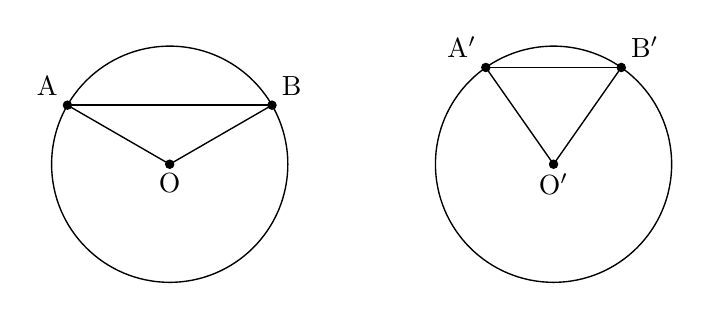
\begin{tikzpicture}[scale=.75]
\tkzSetUpLine[line width=1pt,color=black]
\tkzSetUpPoint[fill=black]

\tkzDefPoints{0/0/B,0/0/C1,6.5/0/OO}
\tkzDefPoints{0/0/O,2/0/X}

\tkzDefPoint(30:2){B}
\tkzDefPoint(150:2){A}

\tkzDrawCircle[color=black,line width=0.5pt,fill=white](O,X)
\tkzDrawSegments[line width=0.5pt,color=black](O,A O,B)
\tkzDrawSegments[line width=0.7pt](A,B)


\tkzDefShiftPoint[OO](55:2){BB}
\tkzDefShiftPoint[OO](125:2){AA}

\tkzDrawCircle[color=black,line width=0.5pt,fill=white](OO,AA)
\tkzDrawSegments[line width=0.5pt,color=black](OO,AA OO,BB)
\tkzDrawSegments[line width=0.7pt](AA,BB)

\tkzDrawPoints[size=3](A,B,O,AA,BB,OO)
\tkzLabelPoint[above left](A){$\rm A$}
\tkzLabelPoint[above right](B){$\rm B$}
\tkzLabelPoint[below](O){$\rm O$}

\tkzLabelPoint[above left](AA){$\rm A'$}
\tkzLabelPoint[above right](BB){$\rm B'$}
\tkzLabelPoint[below](OO){$\rm O'$}

\end{tikzpicture}
\end{document}
